\documentclass[a4paper,10pt]{report}
\usepackage[utf8]{inputenc}
\usepackage{url}
\usepackage[brazil]{babel}
\usepackage{listings}
\usepackage{graphicx}

% Title Page
\title{Tutorial Introdutório ao Google Refine}
\author{Flávio Codeço Coelho \and Renato Rocha Souza}

\lstset{language=python,
        breaklines=true
      }
\begin{document}
\maketitle

\begin{abstract}
Neste tutorial vamos conhecer o Google Refine\footnote{\url{http://code.google.com/p/google-refine}} e aprender a como utilizá-lo na limpeza de conjuntos de dados mal-estruturados e com vários tipos de problemas.
\end{abstract}
\tableofcontents
\chapter{Introdução}
\section{Visão Geral}
O Google Refine é uma ferramenta para lidar com dados de má qualidade, voltada principalmente para ajudar a localiza e consertar inconsistências.
\chapter{Importando Dados}
Para poder analisar dados no Refine é preciso primeiro importá-los. O Refine sabe como ler arquivos nos seguintes formatos:
\begin{itemize}
 \item     TSV, CSV, ou valores separados por um separador especificado por você.
\item Excel (.xls, xlsx)
 \item    XML, RDF com XML
 \item    JSON
 \item    Google Spreadsheets
 \item    RDF triplas N3 
\end{itemize}

O Refine também importa multiplos arquivos compactados com extensões .zip, .tar.gz, .tgz, .tar.bz2, .gz, or .bz2. Neste caso o Refine detecta o tipo de arquivo mais comum e importa todos os dados segundo este formato.

\chapter{Explorando os Dados}
A primeira etapa em qualquer tarefa de análise de dados consiste e nos familiarizar com o conjunto de dados. Para este fim, o Refine oferece algumas ferramentas de exploração de dados que vamos apresentar a seguir.
\section{Facetação}
Facetação refere-se a um conjunto de técnicas que visam resumir um conjuntos por meio de agregação baseada no valor das células de uma coluna.

O tipo mais comum de facetação é por texto. Por exemplo, na tabela de andamentos do Supremo em Números, podemos facetar pela coluna andamento (figura \ref{fig:text_faceting}). Ao fazer isso, temos como resposta um agrupamento pelos valores destas colunas. A esquerda da tela vemos todas as strings distintas que esta coluna apresenta, e podemos então clicar em uma restringir avisualização dos dados a apenas as linhas que possuem aquela string na coluna ``andamento'' (veja figura \ref{fig:text_faceting}).

O refine possui vários tipos de rotinas de facetação pré-programadas (por texto, número, datas, numérica, etc., ver figura \ref{fig:type_facet}) e ainda permite que programemos uma facetação arbitrária. 



\begin{figure}[h!]
 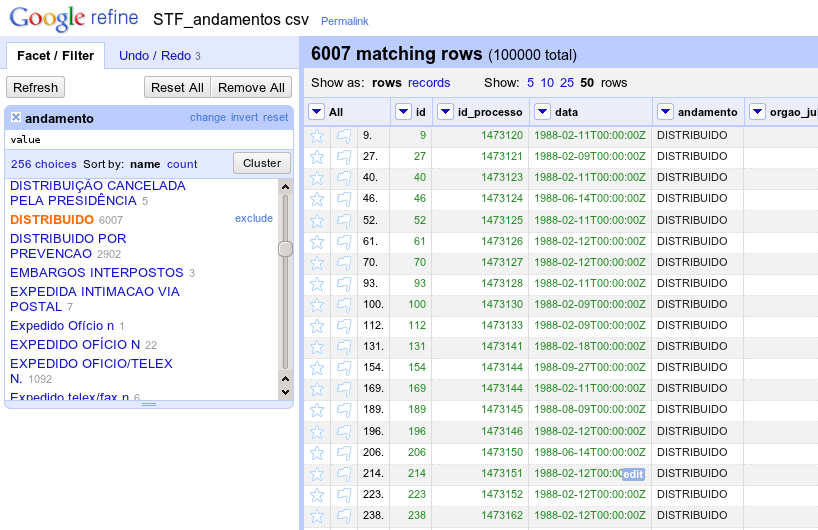
\includegraphics[width=12cm]{./text_faceting.png}
 % text_faceting.png: 818x530 pixel, 95dpi, 21.87x14.17 cm, bb=0 0 620 402
 \caption{Facetação simples por texto.}
 \label{fig:text_faceting}
\end{figure}

Ainda podemos facetar por múltiplas colunas por meio de programação:

\begin{lstlisting}
 cells["andamento"].value[0] == cells["observacao"].value[0]
\end{lstlisting}

O exemplo acima demonstra como podemos facetar agrupando linhas em que a primeira letra é igual de duas colunas de texto é igual.

\begin{figure}[h!]
 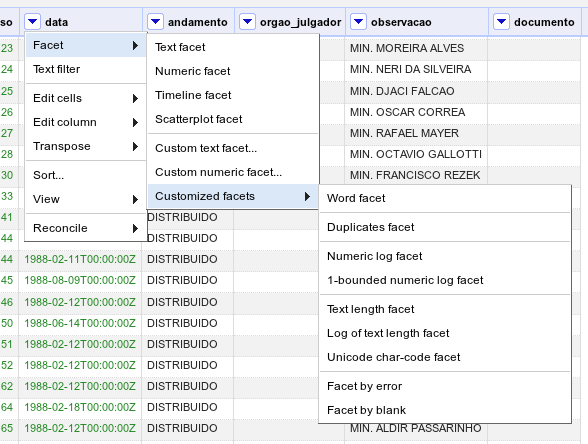
\includegraphics[width=12cm]{./tipos_facet.png}
 % tipos_facet.png: 588x444 pixel, 95dpi, 15.72x11.87 cm, bb=0 0 446 337
 \caption{Tipos de facetação oferecidos pelo Refine}
 \label{fig:type_facet}
\end{figure}



\chapter{Transformando dados}

\section{Transformando Texto}
\subsection{Mascarando dados sensíveis}
Muitas vezes precisamos trabalhar com dados que são confidenciais ou não podem ser revelados a quem precisa analisá-los. Uma técnica matemática  muito eficaz para mascarar textos de forma concisa é a transformação do dado por meio de uma função de embaralhamento (hash) criptográfico.

Segundo a definição da Wikipedia\footnote{http://pt.wikipedia.org/wiki/Função\_de\_embaralhamento\_criptográfico}:

\begin{quote}
A Função de embaralhamento criptográfico é uma procedimento determinístico que leva a um bloco arbitrário de dados e devolve uma cadeia de caracteres de bits com tamanho fixo, o valor (criptográfico) de embaralhamento, de tal forma que uma mudança acidental ou intencional de dados irá alterar o valor do embaralhamento (ver figura \ref{fig:hash}). Os dados a serem codificados muitas vezes são chamados de "mensagem", e o valor de embaralhamento é chamado às vezes de a resumo da mensagem ou simplesmente resumo.\end{quote}

\begin{figure}[h!]
 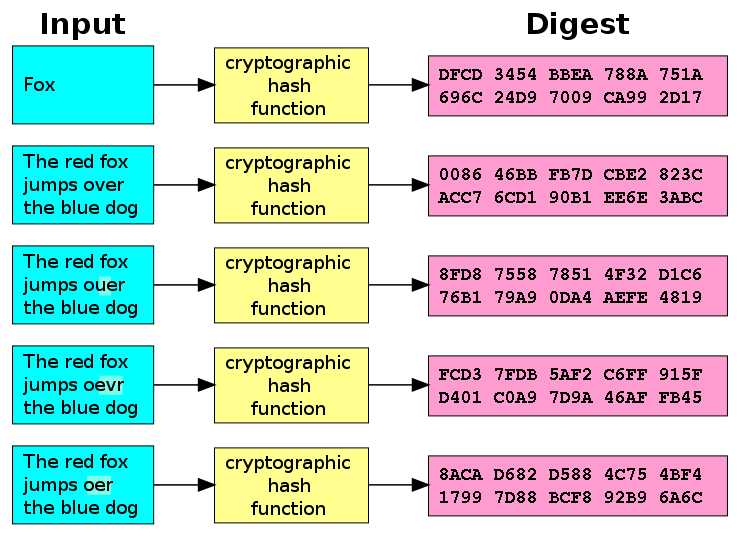
\includegraphics[width=12cm]{./740px-Cryptographic_Hash_Function.png}
 % 740px-Cryptographic_Hash_Function.png: 740x536 pixel, 72dpi, 26.11x18.91 cm, bb=0 0 740 536
 \caption{Uma função criptográfica de embaralhamento (especificamente, SHA-1) funcionando. Note que mesmo pequenas mudanças no código-fonte alteram drasticamente a saída do resultado, pelo chamado efeito avalanche.fonte: Wikipedia}
 \label{fig:hash}
\end{figure}

Usando a linguagem Python, podemos pedir ao Google refine para substituir uma coluna inteira por sua versão embaralhada pela função MD5.


\begin{lstlisting}
import md5;
hash=md5.md5(value)
return hash.hexdigest()
\end{lstlisting}

Veja na figura \ref{fig:hashcode} como implementar esta transformação no Refine. Após selecionar no menu da coluna que se deseja transformar, a opção ``edit cell'' $\mid$ ``transform\ldots'', copie o código Python acima conforme ilustrado na figura \ref{fig:hashcode}, não esquencendo de selecionar Jython no menu ``language''. Finalmente pressione ``OK'' para aplicar o resultado aos seus dados.

\begin{figure}[h!]
 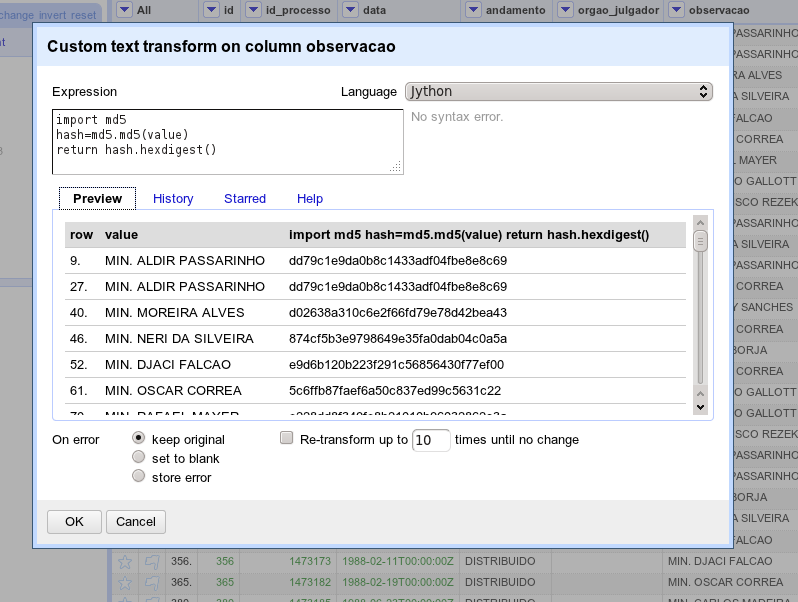
\includegraphics[width=12cm]{./hashing_column.png}
 % hashing_column.png: 798x602 pixel, 95dpi, 21.34x16.10 cm, bb=0 0 605 456
 \caption{substituindo o valor de uma coluna pelo seu MD5 hash}
 \label{fig:hashcode}
\end{figure}

\subsection{Limpando Dados}
\label{sec:limpdados}
Imagine que tenhamos uma coleção de endereços como a mostrada na figura \ref{fig:endsujo}. Note que na coluna endereço,  temos uma mistura de logradouro, com número e salas. Este formato é pouco interessante se desejarmos comparar estes endereços com uma base canônica de endereços, como a dos correios, por exemplo. Vamos ver então como podemos extrair apenas o logradouro e número destes endereços formatados livremente. Como vamos realizar uma edição complexa de texto, convém antes transformar todas as células para caixa alta. Podemos fazer isso com a função ``edit cells'' $\rightarrow$ ``common transforms'' $\rightarrow$ ``to uppercase''.

No menu da coluna endereço vamos selecionar a opção ``edit column'' $\rightarrow$ ``add column based on this column''

\begin{lstlisting}[label=end_limp, caption=codigo Python para limpeza dos endereços]
nv = value.replace(', N.º',',').split('/')[0] 
nv = nv.replace('Nº',',') 
nv = nv.replace('N.º',',') 
nv = nv.replace(', N.',',') 
nv = nv.replace('N.',',') 
nv = nv.replace(', ,',',') 
nv = nv.split('-')[0] 
nv = nv.split('SALAS')[0] 
nv = nv.split('SALA')[0] 
nv = nv.split('SLS')[0] 
return nv
\end{lstlisting}
 
A operação de limpeza exemplificada na listagem \ref{end_limp}, não é perfeita, mas já melhora bastante a qualidade do nosso campo endereço. A figura \ref{fig:limp_end}, mostra-nos como implementar a limpeza.


\begin{figure}[h!]
 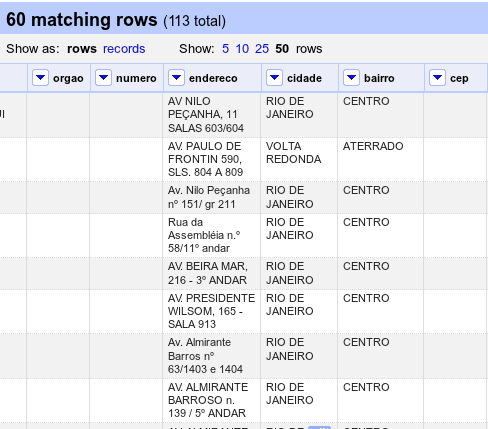
\includegraphics[width=10cm]{./enderecos_sujos.png}
 % enderecos_sujos.png: 488x429 pixel, 95dpi, 13.05x11.47 cm, bb=0 0 370 325
 \caption{Endereços sem normalização}
 \label{fig:endsujo}
\end{figure}

\begin{figure}[h!]
 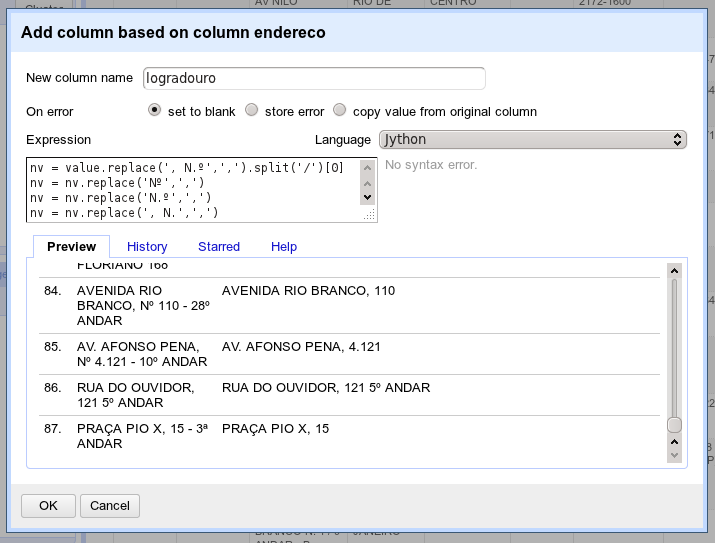
\includegraphics[width=12cm]{./limpeza_end.png}
 % limpeza_end.png: 715x543 pixel, 95dpi, 19.12x14.52 cm, bb=0 0 542 412
 \caption{Criando uma nova coluna "logradouro" baseada na limpeza da coluna endereço.}
 \label{fig:limp_end}
\end{figure}





\chapter{Enriquecendo Dados}
Neste capítulo vamos lidar com técnicas conhecidas no jargão técnico com ``data augmentation''. Estas técnicas consistem em capturar dados de outras fontes  de forma a enriquecer nosso conjunto original de dados. Esta não é uma tarefa simples porém pois os novos dados devem ser pareados com os dados pré-existentes.

\section{Capturando Dados a partir da Web}
Suponhamos que nós temos em uma coluna do nosso banco de dados, endereços. Endereços são um tipo de dado que nos fornece informação com relação à localização espacial de nosso dados mas, se quisermos construir uma visualização espacial destes dados precisaremos de informações mais específicas, como a latitude e longitude destes endereços.

Como podemos tentar resolver este problema no Google Refine?

Na seção \ref{sec:limpdados}, realizamos a limpeza de um conjunto de endereços. Para obter a geolocalização  destes endereços a partir de uma fonte aberta de dados, podemos usar a api do Openstreetmap\footnote{\url{http://nominatim.openstreetmap.org}} (para maiores informações leia documentação\footnote{\url{http://wiki.openstreetmap.org/wiki/Nominatim}})

Para criar uma coluna com as coordenadas dos endereços, precisamos selecionar \emph{``add column by fetching URLs based on column endereço''}.

então digitamos a url que desejamos consultar. No nosso casos é esta.

\begin{lstlisting}[]
'http://nominatim.openstreetmap.org/search?format=json&email=seuemail.gmail.com&q=' + escape(value,'url') + ',' + escape(cells['cidade'].value,'url')
\end{lstlisting}

temos que configurar o campo throttle para no mínimo 1500 milisegundos para evitar recusas no servidor do Openstreetmap. Neste caso utilizaremos a linguagem GREL (Google Refine Expression Language). Vamos nomear a nossa nova coluna de json, pois os dados que vamos receber estão em formato JSON\footnote{JSON: JavaScript Object Notation} Agora clicamos \emph{Ok} e aguardamos o resultado(figura \ref{fig:endjson}). Depois de recebermos os endereços em formato JSON, Necessitamos extrair apenas os dados que queremos: Latitude e Longitude. Para isso vamos usar a opção ``add column based on this column'' da coluna json. Na janela de criação da coluna adicionaremos o seguinte código em GREL:

\begin{lstlisting}[label=lst:parse_end,caption=Extraindo latitudes e longitudes dos endereços em JSON]
 with(value.parseJson()[0],par,par.lat+','+par.lon)
\end{lstlisting}


\begin{figure}[h!]
 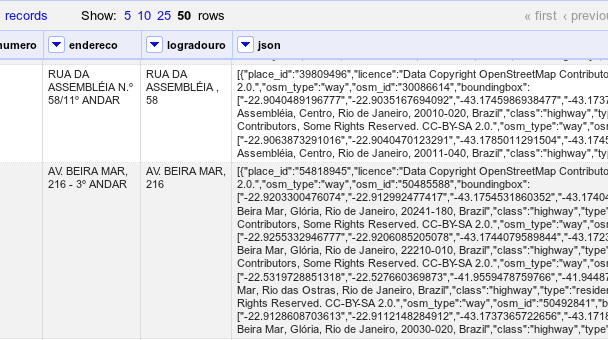
\includegraphics[width=12cm]{./end_json.png}
 % end_json.png: 608x340 pixel, 95dpi, 16.26x9.09 cm, bb=0 0 461 258
 \caption{Resultado da busca no OpenStreetMap}
 \label{fig:endjson}
\end{figure}


A figura \ref{fig:parsejson}, mostra a extração dos valores por meio do código da listagem \ref{lst:parse_end}. 

\begin{figure}[h!]
 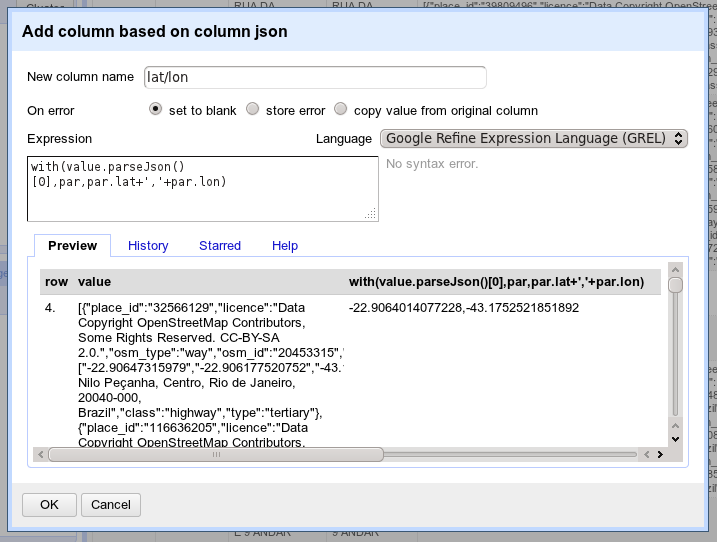
\includegraphics[width=12cm]{./Parse_end_json.png}
 % Parse_end_json.png: 717x542 pixel, 95dpi, 19.17x14.49 cm, bb=0 0 543 411
 \caption{Extraindo latitudes e longitudes dos endereços em JSON}
 \label{fig:parsejson}
\end{figure}

Agora que dispomos das latitudes e logitudes, podemos exportar nossa tabela e preparar uma visualização dos nossos dados usando, por exemplo, outra ferramenta gratuita, o Google Fusion Tables(figura \ref{fig:fusiont}).

\begin{figure}[h!]
 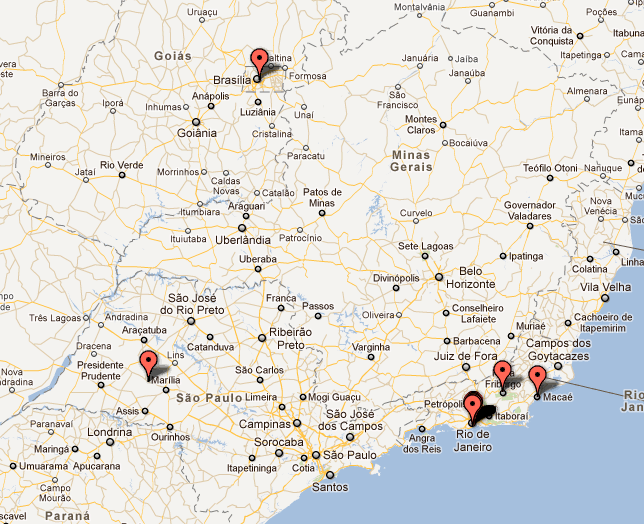
\includegraphics[width=12cm]{./fusiontables.png}
 % fusiontables.png: 644x524 pixel, 95dpi, 17.22x14.01 cm, bb=0 0 488 397
 \caption{Visualização dos endereços geo-localizados no Fusion Tables}
 \label{fig:fusiont}
\end{figure}


\end{document}          
